%!TEX root = paper.tex
\section{Overview}\label{sec-overview}

\gls{oin}, Vienna's community-operated \gls{IoT} network, hinges on
three architectural elements supporting its operation:
First, the wireless connectivity between sensors and the network
uses \gls{lora} and \gls{lorawan} specifically.
Second, the gateways and backend operate according to the architecture
proposed by \gls{ttn}~\cite{ttn}.
Third, gateways, backend, Internet connectivity etc. are built, operated,
maintained, and contributed by volunteer community members of \gls{oin},
all under the premise that the system is open to the public for use and
contributions on all layers.
In the following, we describe each aspect in greater detail.


\subsection{\gls{lora} and \gls{lorawan}}

\gls{lora} is a proprietary layer-1 technology for low-power long-range
low-bandwidth wireless transmissions. It operates in license-exempt
frequency ranges (the 433 MHz (EMEA, northern Asia) and 915 MHz
(the Americas) \acrshort{ISM} bands, and the European 868 MHz
\acrshort{SRD} band). The transmit power is thus limited to around
10 dBm (10 milliwatts), depending on local legislation.
\gls{lora} symbols consist of constant-amplitude up- and downchirps,
with an overall configurable chirp rate (called ``spreading factor'')
and bandwidth.
A certain degree of orthogonality between temporally overlapping
transmissions is achieved by using different sub-ranges of
the current frequency band (better), and assigning different spreading
factors to different senders (less optimal)~\cite{croce}.
Otherwise, senders are assumed to listen-before-talk, use low
transmit power, and limit their active duty cycles explicitly
according to radio regulations in the frequency band, and implicitly
due to limited available (battery) power.
Depending on the actual modulation parameters used, \gls{lora}
achieves bit rates of 300-21,000 bits per second, and message lengths
of 20 to 250 bytes.
% Sensitivity -148 dBm, https://www.microchip.com/design-centers/wireless-connectivity/low-power-wide-area-networks/lora-technology
%
% Message length on the air 50-1500 ms

\gls{lorawan}~\cite{lorawan-specs} builds on \gls{lora} and adds
a message format usable in a system with wireless end devices,
access gateways, and network servers for further data processing.
The message format
supports two layers of AES-128 cryptography to secure
the message contents. A Network Session Key is used to calculate a
message integrity code, and to encrypt MAC-only (i.e., not
application-oriented) messages. The Application Session Key encrypts
application-specific messages. Both session keys may derived in an
over-the-air activation procedure that assumes a pre-shared
Application Identifier (AppEUI) to be present in the device.
In addition, the device's globally unique EUI-64 address is used
for session key derivation. Thus, every device derives its own
application- and device-specific Network and Application session key,
and key compromise only affects that single device.
Besides, the message format supports framing information, managing
endpoint addressing, acknowledgement requests and retransmissions,
data rate adaptations, etc.


\subsection{\gls{ttn}'s system architecture}

\gls{oin}'s deployment is built on \gls{ttn}'s system architecture~\cite{ttn}.
It interfaces with other compatible systems around the world.
Figure~\ref{fig:ttn-arch} overviews the system architecture employed
by \gls{ttn}. Wireless devices (left) transmit messages that are
received by one or more gateways. Network servers manage the gateways,
balance their utilization, track device states, forward server traffic
for specific applications over the Internet, and support service discovery.

Remarkably, the \gls{ttn} system architecture roots in the assumption
that services are distributed across domains and are contributed
by multiple parties. No single operator controls the network.
Therefore, implicit trust must be minimized, and clear, functional
component separations emerge.
This is in contrast to the operator-centric notion of traditional
communication networks.

\begin{figure}
  \centering
  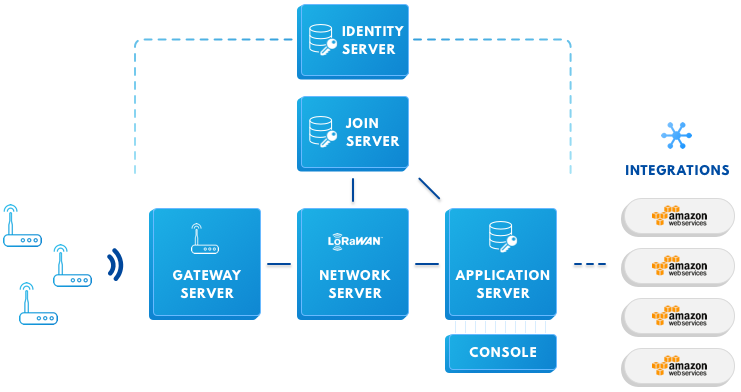
\includegraphics[width=\columnwidth]{figures/ttn_tech_stack.png}
  \caption{\gls{ttn}'s system architecture~\cite{ttn}.}
  \label{fig:ttn-arch}
\end{figure}


\subsection{The \gls{oin} community}

Vienna's local \gls{ttn} chapter currently has about forty members
registered, with 20 registered gateways. The \gls{oin} community
overall is about five times that size, counting both regulars and
more loosely associated enthusiasts. Note that \gls{oin} requires
no formal membership to participate in the project, join community
meetings, or use and contribute sensors, gateways, and the network.
Contributors not only include wirelessly inclined people from the
local amateur radio and community wireless populace, industry,
schools, academia, and municipality, but also from the general
public (with no specific background in the technical field).
The applications and uses of \gls{oin} parallel the diversity
of its contributors, and mutual inspiration results from it.
Similarly, \gls{oin}'s gateways are hosted both at sites set up
previously in other wireless-related contexts, and new sites
made available by contributors recently attracted to the project.
